%\subsection{Strain Gauge}
\indent The deformation and displacement that an object feels under an external force is defined as strain \cite{OmegaEngineeering:2013}. In the applications of engineering and construction the strain of an object, such as a support or beam, is a necessary component to monitoring the structure. To measure the strain of a structure, a strain gauge may be applied. The strain gauge can be a very effective measurement technique for SHM because it has the ability to measure the compression and expansion within the members of the structure. The strain values measured on the structure can be used to state the stress within the material to monitor and predict the safety of the structure. The change in capacitance, inductance or resistance is proportional to the strain experienced by the sensor. The strain sensitivity or gauge factor is a dimensionless figure that represents the tolerance of the gauges . It allows for the gauge to have minimal imprecision for changes in temperature. Equation \ref{eqn:Strain_GaugeFactor} shows the calculation of the gauge factor (GF) for a strain gauge

\begin{equation}
GF = \frac{\Delta R / R}{\epsilon} 
\label{eqn:Strain_GaugeFactor}
\end{equation}
\indent Where $\epsilon$ is the lateral or longitudinal strain; defined by \ref{eqn:Strain_StrainEqn}.

\begin{equation}
\epsilon = \frac{\Delta L}{L}
\label{eqn:Strain_StrainEqn}
\end{equation} 

\indent Ideally strain would only change due to a change to the surface on which the sensor is attached to. However, temperatures, material properties, the bonding adhesive and the stability of the metal all affect the detected resistance. So when selecting a strain gage one must be thorough in understanding the conditions the gage may be under during use. Because material properties are not the same in each direction, knowing axial strain is not sufficient. Poisson strain and shearing strain of the material are required to calculate the principal strain. Poisson strain is both the thinning and widening of the beam, as well as the elongation that the beam may feel under strain. Shearing strain is the angular distortion of the beam, or the angle of rotation or twist due to shear stress. Generally, to calculate the principal strains the largest normal strain is of most interest. This can be found by taking the derivative of $\epsilon X$ or $\epsilon Y$ with respect to $\theta$ and equating it to zero. This gives the principal rotation angle, $\theta p$, this will help produce the principal strains (max and min); as seen in Equations \ref{eqn:Strain_Ep} - \ref{eqn:Strain_Theta}
\begin{equation}
\epsilon_{p,q} = \frac{1}{2}\biggl[\epsilon_{1} + \epsilon_{3} \pm \sqrt{(\epsilon_{1}-\epsilon_{3})^{2}+(2\epsilon_{2}-\epsilon_{1}-\epsilon_{3})^{2}}\biggr]
\label{eqn:Strain_Ep}
\end{equation}

\begin{equation}
\sigma_{p,q} = \frac{E}{2}\biggl[\frac{\epsilon_{1}+\epsilon_{3}}{1-\nu}\pm \frac{1}{1+\nu}\sqrt{(\epsilon_{1}-\epsilon_{3})^{2}+(2\epsilon_{2}-\epsilon_{1}-\epsilon_{3})^{2}}\biggr]
\label{eqn:Strain_Sig}
\end{equation}

\begin{equation}
\Theta_{p,q} = \frac{1}{2} \tan^{-1}\biggl(\frac{2\epsilon_{2}-\epsilon_{1}-\epsilon_{3}}{\epsilon_{1}-\epsilon_{3}}\biggr)
\label{eqn:Strain_Theta}
\end{equation}

\noindent The towers of the Newport Bridge stand 400 feet tall, the suspended structure consists of over 23,000 tons of steel, the total length of the wires is close to 8,000 miles, and the amount of concrete used in the substructure is 136,000 cubic yards \cite{Structurae:2013}. There are many aspects of the bridge that can be damaged; the best process to minimize the damages that may occur is to inspect the structure as often as possible and make repairs in a timely manner. Implementing strain gauges to monitor the structural health of the bridge is the most economical procedure to continually collect data to assess if structural changes have occurred. For the design group to collect accurate strain measurements that can be analyzed to assess the bridge's health, bonded foil strain gauges were used. Imaged below is a figure of a 3-element strain gauge. 

\begin{figure}[H]
\centering
\includegraphics*[width =3in]{OMEGA_Rose}
\caption{\textit{3-Element Rosette, metal-foil type strain gauge\\Manufacturer: Omega}}
\label{fig:STRAIN_Rose}
\end{figure}

\indent The typical metal foil-type strain gauge consists of a grid of wire filament that acts as a variable resistor. The gauge is bonded onto the surface of the structure by using an epoxy resin specific to the structure material. When the structure is under strain the change in surface length results in a change in the resistance, this change in electrical resistance in the foil varies linearly with strain. To obtain strain with a metal foil-type strain gauge a Wheatstone bridge must be utilized to measure the small changes in resistance due to strain. A Wheatstone bridge is a divided bridge circuit used for measuring static or dynamic electrical resistance. The Wheatstone Bridge utilizes the difference in resistance from each half of the bridge to either produce a voltage differential when measured from one half of the bridge to the next.


\begin{figure}[H]
\centering
\includegraphics*[width =3in]{Strain_Wheat}
\caption{\textit{Wheatstone Bridge Circuit Schematic}\cite{OmegaEngineeering:2013}}
\label{fig:STRAIN_Wheat}
\end{figure}

\indent For the sensor to accurately measure the strain of the proposed test beam, the group needed a 3-element rosette with a nominal resistance of $120\Omega$, max permitted bridge energizing voltage of $12V_{rms}$ that was matched to aluminum, and a maximum strain of 30,000 micro strain ($\mu \epsilon$). The strain gauge originally selected was the SGD-6/120-RYT83.

\subsection{Strain Gauge Selection}
\indent The primary factors that influenced the strain gauge selection were:

\begin{itemize}
\item Operating Temperature
\item State of Strain
\item Stability of the Metal Foil
\item Gauge Factor
\item Power Consumption
\end{itemize}

\paragraph{Operating Temperature}
\indent The service temperature of the strain gauges needed for our project must be versatile. The service temperature for the gauges purchased range from $-100^{\circ}$F to $392^{\circ}$F. 
\paragraph{State of Strain}
\indent The nature of the strain for this project was mostly axial strain. There was also bending strain from the force of the load applied during testing as well as shear strain determined by measuring the strain at a $45^{\circ}$ angle. The 3-element rosette allowed for the sensor to measure all three types of strain at once.
\paragraph{Stability of the Metal Foil}
\indent The stability of the metal foil measuring grid is important because the electrical resistance must be measured accurately on a consistent basis. The strain gauge applied in this project uses a 5-micron thick constantan foil. Constantan is a copper, nickel alloy that is most often the type of metal foil used within a strain gauge because of its consistent gauge factor which is highly dependent on temperature with other metal foils such as Karma which is a nickel, chromium alloy.
\paragraph{Gauge Factor}
\indent The gauge factor or strain sensitivity of a sensor is the proportionality factor between the relative change in resistance . The gauge factor chosen varies less with change in temperature than other types of gauges, this can be seen by viewing the Copper Nickel curve in Figure \ref{fig:STRAIN_GFvT}. The sensor used for the package had a gauge factor of 2.0.

\begin{figure}
\centering
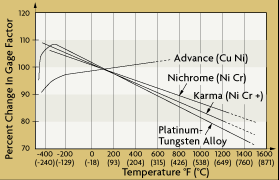
\includegraphics[scale=1]{STRAIN_PercentTemp}
\caption{\textit{Graph showing the relationship between gauge factor and temperature change}\cite{OmegaEngineeering:2013}}
\label{fig:STRAIN_GFvT}
\end{figure}

\paragraph{Power Consumption}
\indent The power consumption of the gauge is mostly a result of the needed connection to the Wheatstone Bridge. The quarter bridge circuit consumes $27.5 mA$ at $3.3V$, or $90.8mW$.



\begin{figure}[H]
\centering
\includegraphics*[width =3in]{OMEGA_Soldered}
\caption{\textit{Omega 3-Element Rosette with leads attached}}
\label{fig:Soldered Strain Gauge}
\end{figure}

\indent Figure \ref{fig:Soldered Strain Gauge} pictured above is the one of the original 3-element rosette strain gauges with wires soldered to the solder pads. Due to the small solder pads, it proved to be difficult to achieve secure solder joints. It is likely that the gauges were damaged upon soldering the wires to them because of the poor data that was collected from them. To arrest these issues the group purchased strain gauges with the leads directly connected to the solder pads. Purchased from omega engineering, the model number was SGD-6/120RYT23. These gauges included ribbon leads, however when attaching clips to the leads during experimentation the leads came undone. Despite the troublesome attempts to get the strain gauges working, once they were connected correctly there was still no accurate data received. A strain gauge with a different gague factor or a higher resistance would be more appropiate.
